\section{Modelo del Negocio}
Antes de especificar el software, se modela el funcionamiento de la agencia PERÚ TOURS siguiendo la metodología de Jesús García Molina et al.~\cite{garciamolina} % Cita: Paper metodológico "De los Procesos del Negocio a los Casos de Uso" (Univ. de Murcia)
. Esto permite alinear los objetivos comerciales, los participantes y los procesos operativos antes de construir el sistema.

\subsection{Objetivos del Negocio (ON)}
Se definen las metas estratégicas que la agencia busca alcanzar con la optimización de sus procesos:
\begin{itemize}[noitemsep]
    \item \textbf{ON-01 (Agilidad):} Reducir el tiempo de armado y entrega de cotizaciones a menos de 4 horas hábiles.
    \item \textbf{ON-02 (Crecimiento):} Aumentar la afiliación de nuevos socios en un 40\% durante el primer año.
    \item \textbf{ON-03 (Conversión):} Recuperar al menos el 25\% de cotizaciones observadas mediante un reajuste ágil de presupuestos.
    \item \textbf{ON-04 (Control):} Lograr el 100\% de registro y trazabilidad de cotizaciones canceladas u observadas para la toma de decisiones gerenciales.
\end{itemize}

\subsection{Actores y Trabajadores del Negocio}
Siguiendo la notación formal de RUP, se diferencian los roles externos de los internos:
\begin{itemize}
    \item \textbf{Actores de Negocio (\texttt{<<Business Actor>>}):} 
    \begin{itemize}[noitemsep] 
        \item \textbf{AN-01 Cliente Turista:} Usuario externo que solicita cotizaciones a medida, negocia cambios y contrata el paquete de viaje.
        \item \textbf{AN-02 Pasarela Bancaria:} Entidad financiera externa encargada de procesar, validar y liquidar los cobros electrónicos.
    \end{itemize}
    \item \textbf{Trabajadores de Negocio (\texttt{<<Business Worker>>}):}
    \begin{itemize}[noitemsep]
        \item \textbf{TN-01 Agente Receptivo:} Operador interno responsable de estructurar las cotizaciones, ajustar costos según observaciones y atender al socio.
        \item \textbf{TN-02 Gerente de Agencia:} Directivo interno responsable de auditar operaciones, revisar cotizaciones canceladas y analizar el desempeño comercial.
    \end{itemize}
\end{itemize}

\subsection{Casos de Uso del Negocio (CUN) y Diagrama}
Representan los procesos fundamentales que aportan valor directo a la organización:

\begin{itemize}[noitemsep]
    \item \textbf{CUN-01: Afiliar Cliente a Socio:} Permite a un turista nuevo registrarse formalmente para acceder a presupuestos y beneficios de socio.
    \item \textbf{CUN-02: Cotizar Paquete Turístico:} Captura los requerimientos del viaje y genera la propuesta económica por parte del agente.
    \item \textbf{CUN-03: Gestionar Venta y Pago de Paquete:} Conduce la negociación de observaciones, la aprobación formal del presupuesto y el cobro en línea.
    \item \textbf{CUN-04: Auditar y Controlar Cotizaciones:} Proceso gerencial para filtrar y evaluar cotizaciones canceladas o modificadas por rango de fechas.
\end{itemize}

\begin{figure}[H]
    \centering
    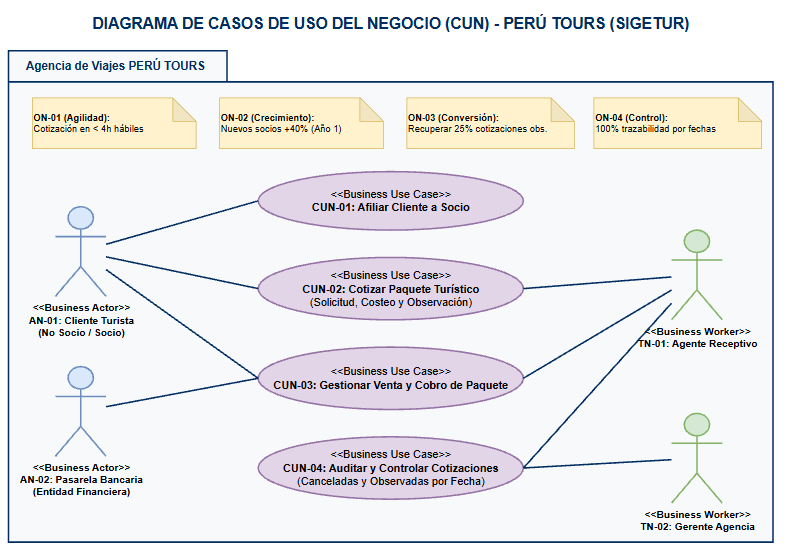
\includegraphics[width=0.85\textwidth]{../diagramas/diagram_cun.png}
    \caption{Diagrama de Casos de Uso del Negocio (CUN) para PERÚ TOURS.}\label{fig:cun}
\end{figure}

\subsection{Diagrama de Actividades con Carriles (Swimlanes)}
El diagrama de actividades detalla la interacción cronológica entre los actores y trabajadores del negocio, separando las responsabilidades por carriles:

\begin{figure}[H]
    \centering
    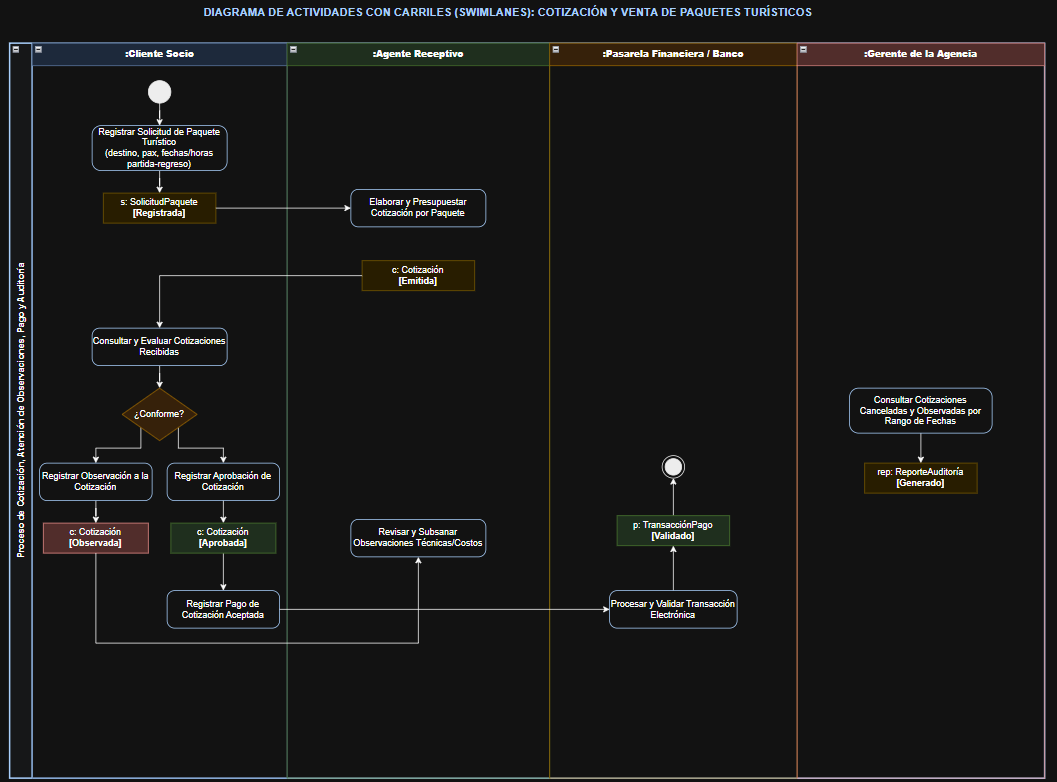
\includegraphics[width=0.88\textwidth]{../diagramas/diagram_actividades.png}
    \caption{Diagrama de Actividades con Carriles y Estados de Objetos del Negocio.}\label{fig:swimlanes}
\end{figure}

\subsubsection{Flujo y Máquina de Estados del Objeto Cotización}
Durante la ejecución de las actividades, el objeto de negocio central \texttt{c: Cotización} transita por los siguientes estados:

\begin{center}
\texttt{[Emitida]} $\longrightarrow$ \texttt{[Observada]} $\rightleftharpoons$ \texttt{[Reajustada]} $\longrightarrow$ \texttt{[Aprobada]} $\longrightarrow$ \texttt{[Pagada]} \quad \text{o bien} \quad $\longrightarrow$ \texttt{[Cancelada]}
\end{center}
\begin{itemize}[noitemsep]
    \item Si el cliente acepta la cotización emitida, pasa de inmediato a \texttt{[Aprobada]} y queda habilitada para el cobro (\texttt{[Pagada]}).
    \item Si el cliente solicita modificaciones, pasa a \texttt{[Observada]}, obligando al agente a generar una versión \texttt{[Reajustada]} hasta lograr la aprobación o llegar a su anulación definitiva (\texttt{[Cancelada]}).
\end{itemize}